% Options for packages loaded elsewhere
\PassOptionsToPackage{unicode}{hyperref}
\PassOptionsToPackage{hyphens}{url}
%
\documentclass[
  answers,addpoints,12pt]{exam}
\usepackage{amsmath,amssymb}
\usepackage{lmodern}
\usepackage{iftex}
\ifPDFTeX
  \usepackage[T1]{fontenc}
  \usepackage[utf8]{inputenc}
  \usepackage{textcomp} % provide euro and other symbols
\else % if luatex or xetex
  \usepackage{unicode-math}
  \defaultfontfeatures{Scale=MatchLowercase}
  \defaultfontfeatures[\rmfamily]{Ligatures=TeX,Scale=1}
\fi
% Use upquote if available, for straight quotes in verbatim environments
\IfFileExists{upquote.sty}{\usepackage{upquote}}{}
\IfFileExists{microtype.sty}{% use microtype if available
  \usepackage[]{microtype}
  \UseMicrotypeSet[protrusion]{basicmath} % disable protrusion for tt fonts
}{}
\makeatletter
\@ifundefined{KOMAClassName}{% if non-KOMA class
  \IfFileExists{parskip.sty}{%
    \usepackage{parskip}
  }{% else
    \setlength{\parindent}{0pt}
    \setlength{\parskip}{6pt plus 2pt minus 1pt}}
}{% if KOMA class
  \KOMAoptions{parskip=half}}
\makeatother
\usepackage{xcolor}
\usepackage[top=1.5cm,bottom=1.5cm,left=1.5cm,right=1.5cm]{geometry}
\usepackage{longtable,booktabs,array}
\usepackage{calc} % for calculating minipage widths
% Correct order of tables after \paragraph or \subparagraph
\usepackage{etoolbox}
\makeatletter
\patchcmd\longtable{\par}{\if@noskipsec\mbox{}\fi\par}{}{}
\makeatother
% Allow footnotes in longtable head/foot
\IfFileExists{footnotehyper.sty}{\usepackage{footnotehyper}}{\usepackage{footnote}}
\makesavenoteenv{longtable}
\usepackage{graphicx}
\makeatletter
\def\maxwidth{\ifdim\Gin@nat@width>\linewidth\linewidth\else\Gin@nat@width\fi}
\def\maxheight{\ifdim\Gin@nat@height>\textheight\textheight\else\Gin@nat@height\fi}
\makeatother
% Scale images if necessary, so that they will not overflow the page
% margins by default, and it is still possible to overwrite the defaults
% using explicit options in \includegraphics[width, height, ...]{}
\setkeys{Gin}{width=\maxwidth,height=\maxheight,keepaspectratio}
% Set default figure placement to htbp
\makeatletter
\def\fps@figure{htbp}
\makeatother
\setlength{\emergencystretch}{3em} % prevent overfull lines
\providecommand{\tightlist}{%
  \setlength{\itemsep}{0pt}\setlength{\parskip}{0pt}}
\setcounter{secnumdepth}{-\maxdimen} % remove section numbering
% \usepackage{exam}

\newcommand{\bquestions}{\begin{questions}}
\newcommand{\equestions}{\end{questions}}
\newcommand{\bsolution}{\begin{solution}}
\newcommand{\esolution}{\end{solution}}
\newcommand{\bparts}{\begin{parts}}
\newcommand{\eparts}{\end{parts}}
\newcommand{\stpart}{\part} % this is absolutely necessary to make new part command
\newcommand{\bsubparts}{\begin{subparts}}
\newcommand{\esubparts}{\end{subparts}}
\newcommand{\stsubpart}{\subpart}

% solution environment is a minipage and cannot support float so, always use "HOLD_position" 
\usepackage{float} % this package is essential for solution with code
% eqnarray is better avoided, most suggestion lead to \align provided in amsmath
% also split is used when there are very long lines of equation
% for different expression of the same equation use line separator \\ and use \notag or \nonumber
\usepackage{eqnarray, amsmath}

% \usepackage{background}
% \usepackage{eso-pic}
% \usepackage{contour}
% 
% \backgroundsetup{
%   angle=90,
%   opacity=0.8,
%   scale=1.2,
%   color=red,
%   nodeanchor=south west,
%   position={current page.south east},
%   contents={}{{\footnotesize Generated by }{\Large Deependra Dhakal }{(\footnotesize to be shared and distributed freely!)}},
%   hshift=40pt,% to move the text vertically
%   vshift=+10pt% to move the text horizontally
% }
% 
% \pagestyle{empty}

\newcommand{\under}[1]{%
  \vphantom{#1}%
  \underaccent{\bar}{\smash[b]{#1}}%
  }

\newcommand{\probP}{\text{I\kern-0.12em P}}
\usepackage{wasysym}
\usepackage{caption}
\usepackage{booktabs}
\usepackage{longtable}
\usepackage{array}
\usepackage{multirow}
\usepackage{wrapfig}
\usepackage{float}
\usepackage{colortbl}
\usepackage{pdflscape}
\usepackage{tabu}
\usepackage{threeparttable}
\usepackage{threeparttablex}
\usepackage[normalem]{ulem}
\usepackage{makecell}
\usepackage{xcolor}
\ifLuaTeX
  \usepackage{selnolig}  % disable illegal ligatures
\fi
\IfFileExists{bookmark.sty}{\usepackage{bookmark}}{\usepackage{hyperref}}
\IfFileExists{xurl.sty}{\usepackage{xurl}}{} % add URL line breaks if available
\urlstyle{same} % disable monospaced font for URLs
\hypersetup{
  pdftitle={Probability for Genetics and Plant Breeding},
  hidelinks,
  pdfcreator={LaTeX via pandoc}}

\title{Probability for Genetics and Plant Breeding}
\usepackage{etoolbox}
\makeatletter
\providecommand{\subtitle}[1]{% add subtitle to \maketitle
  \apptocmd{\@title}{\par {\large #1 \par}}{}{}
}
\makeatother
\subtitle{Numerical Exercises}
\author{Deependra Dhakal}
\date{}

\begin{document}
\maketitle

\hypertarget{probability-in-genetics-and-plant-breeding}{%
\section{Probability in Genetics and Plant Breeding}\label{probability-in-genetics-and-plant-breeding}}

\bquestions

\question \label{quest:genprob1-1}

A blue-eyed and right-handed man had married a dark-eyed right-handed woman. One of their 3 children is blue-eyed and right-handed, while the other two are dark-eyed and left-handed. The man marries again. This time he has right-handed and dark-eyed wife. They have 11 children, all right-handed and dark-eyed. What are probable genotypes of the husband and his wives.

\bsolution (Question \ref{quest:genprob1-1})

Based on generalization about the nature of human body, there are fewer left-handed people among us than are the right handed. Right-handedness is a dominant trait (conditioned by \(R\) allele), and the left-handedness is recessive trait (conditioned by \(r\) allele). The dark eyes, \(D\) allele, are dominant over blue eyes (\(d\) allele). Thus, the genotype of the man is most likely \(R\_dd\). Both wives were right-handed and dark-eyed (dominant traits): \(R\_D\_\).

Man has one right-handed, blue-eyed child (\(R\_dd\)) and two left-handed, dark-eyed children (\(rrDd\)) from first marriage. The only way to have a left-handed child is if both parents have a left-handed allele, \(r\). So, parents in first marriage are heterozygous with respect to handedness (\(Rr\)). The only way to produce a blue-eyed child is if both parents posses a blue-eyed allele, \(d\). Thus, first wife must be heterozygous with respect to eye color (\(Dd\)). The father's eye color genotype is \(dd\). Therefore the genotypes must have been as follows: man -- \(Rrdd\), first wife -- \(RrDd\)

The second marriage produced 11 right-handed and dark-eyed children. If new wife were heterozygous for either character, chances of recessive phenotype occuring existed. However, none of the recessive traits were exhibited in offspring. Taking this fact into account, the second wife must be homozygous dominant for both characters (\(RRDD\)).

\esolution

\question \label{quest:genprob1-2}

Large eyes and thick lips are dominant traits. A man with small eyes and thin lips have wife with large eyes and thick lips. They have a son with large eyes and thick lips. Son married a woman with large eyes and thin lips. They produced 2 children -- Boys with large eyes and thin lips and girl with small eyes and thick lips. Determine the genotypes of all the parents.

\bsolution (Question \ref{quest:genprob1-2})

Let us use following symbology to represent the dominance and recessive forms of alleles:

\begin{itemize}
\tightlist
\item
  Large eyes: \(E\)
\item
  Small eyes: \(e\)
\item
  Thick lips: \(L\)
\item
  Thin lips: \(l\)
\end{itemize}

\[
\begin{aligned}
&\text{Parents:}& &E\_L\_& &\times& &eell& \\
&& &\female& && &\male& \\
&\text{Gametes:}& &EL \text{ or } El \text{ or } eL \text{ or } el& && &el& \\
&\text{Son:}& && &EeLl& && \\
\end{aligned}
\]

\begin{longtable}[t]{lllll}
& $Eell$ (Son's wife) &  & $EeLl$ (Son) & \\
& $\female$ & x & $\male$ & \\
Gametes: & $El, el$ &  & $EL, eL, El, el$ & \\
Children: & \female$eeLl$ &  & \male$E\_ll$ & \\
\end{longtable}

\(\therefore\) The parents from this family have following genotypes:

\begin{itemize}
\tightlist
\item
  Man: \(eell\)
\item
  Wife: \(E\_L\_\)
\item
  Son: \(EeLl\)
\item
  Son's wife: \(Eell\)
\end{itemize}

\esolution

\question \label{quest:genprob1-3}

Sickle cell anemia and talasemia are inherited as incomplete dominance traits. Homozygous individuals die early, while individuals heterozygous on both genes are viable and have a special form of haemoglobin. Malarial plasmodium is not able to feed on this haemoglobin, so heterozygotes do not get sick with malaria. Double heterozygotes develop mild, non-manifested (microdrepanocytary) anaemia. What is the probability of healthy child birth in a family where one parent is heterozygous in respect to sickle cell anemia but normal on talasemia and other is normal with respect to sickle cell anaemia, but heterozygous on talasemia.

\bsolution (Question \ref{quest:genprob1-3})

Let us refer to the conditions with symbology,

\begin{itemize}
\tightlist
\item
  S: Sickle cell anaemia
\item
  A: Absence of sickle cell anaemia (In reality, ``A'' is dominant over ``S'')
\item
  T: Talasemia
\item
  B: Absence of talasemia
\end{itemize}

Independently, diploid phenotypes for each genetic loci exhibits following conditions:

\begin{itemize}
\tightlist
\item
  SS: Severe SC anaemia
\item
  SA: Light, non-clinical form of anaemia
\item
  AA: No anaemia
\item
  TT: Severe talasemia
\item
  TB: Light, non-clinical form of talasemia
\item
  BB: No talasemia
\end{itemize}

The parental cross suggested above can be written as: \(\female SABB \times AATB\). Taken that the genes assort independently, we can illustrate the gametic fusion in punnet square as follows.

\begin{longtable}{>{\raggedright\arraybackslash}p{3em}>{\raggedright\arraybackslash}p{12em}>{\raggedright\arraybackslash}p{12em}}
\toprule
M/F & SB & AB\\
\midrule
AT & SATB, 25\%, light form of both diseases & AATB, 25\%, light form of talasemia, no anaemia\\
AB & SABB, 25\%, light form of anaemia, no talesima & AABB, 25\%, healthy with respect to both diseases but not resistant to malaria\\
\bottomrule
\end{longtable}

\(\therefore\) The probability of a healthy child free of extreme cases of either of two conditions is 25\%.

\esolution

\question \label{quest:genprob1-4}

In human some forms of short-sightedness dominate over normal vision and brown eyes dominate over the blue. Genes of both pairs of traits are situated in different chromosomes. What children can be expected from parents, which are heterozygous for both genes ?

\bsolution (Question \ref{quest:genprob1-4})

Let us, for convenience, take following symbology to represent different conditions:

\begin{itemize}
\tightlist
\item
  S: Short-sightedness
\item
  s: Normal vision
\item
  B: Brown eyes
\item
  b: Blue eyes
\end{itemize}

\begingroup\fontsize{8}{10}\selectfont

\begin{longtable}[t]{>{\raggedright\arraybackslash}p{2em}>{\raggedright\arraybackslash}p{2.5em}>{\raggedright\arraybackslash}p{2.5em}>{\raggedright\arraybackslash}p{2.5em}>{\raggedright\arraybackslash}p{2.5em}}
\caption{\label{tab:unnamed-chunk-1}This phenomena is also known as dominant epistasis, in that one of the two genes shows epistatic action on other when present in dominant state. Gene 'S' is epistatic to gene 'B'. 'S' masks the effect of 'B' with its own phenotype when they both occur together, while B, on its own, shows distinct phenotype.}\\
\toprule
Gamete & SB & Sb & sB & sb\\
\midrule
SB & \cellcolor{red!80}{SBSB} & \cellcolor{red!80}{SBSb} & \cellcolor{red!80}{SBsB} & \cellcolor{red!80}{SBsb}\\
Sb & \cellcolor{red!80}{SbSB} & \cellcolor{red!80}{SbSb} & \cellcolor{red!80}{SbsB} & \cellcolor{red!80}{Sbsb}\\
sB & \cellcolor{red!80}{sBSB} & \cellcolor{red!80}{sBSb} & \cellcolor{green!10}{sBsB} & \cellcolor{green!10}{sBsb}\\
sb & \cellcolor{red!80}{sbSB} & \cellcolor{red!80}{sbSb} & \cellcolor{green!10}{sbsB} & \cellcolor{blue!90}{sbsb}\\
\bottomrule
\end{longtable}
\endgroup{}

From the Punnet square, we observe that 3 of 4 genotypes providing normal vision have brown eyes. The genotype \(ssbb\) provides information for blue eyes and normal vision. All other genotypes (12) code for the short-sightedness: 3 with blue eye color and 9 with brown eye color.

\esolution

\question \label{quest:genprob1-5}

How often in families of 3 children where both parents are heterozygous for non-red hair (\(Rr\)) and have wavy hair (\(h_1h_2\)) will children be

\begin{enumerate}
\def\labelenumi{\roman{enumi}.}
\tightlist
\item
  a red haired girl, a non-red curly haired boy and a red straight haired girl ?
\item
  two red wavy haired boy and one non-red straight haired girl ?
\end{enumerate}

\bsolution (Question \ref{quest:genprob1-5})

Given,

\begin{itemize}
\tightlist
\item
  Total number of children (\(n\)): 3
\item
  Non-red hair genotype: \(Rr\)
\item
  Straight hair genotype: \(h_1h_1\)
\item
  Wavy hair genotype: \(h_1h_2\)
\item
  Curly hair genotype: \(h_2h_2\)
\item
  Dominance relation follows: non-Red (\(R\)) \textgreater{} Red (\(r\))
\end{itemize}

\[
\begin{aligned}
&\female &\times &\male\\
&Rr,h_1h_2 & & Rrh_1h_2
\end{aligned}
\]

Segregation follows,

\begin{itemize}
\tightlist
\item
  At ``R'' loci: \(\frac{1}{4}RR: \frac{2}{4}Rr: \frac{1}{4}rr\) (3 Non-red, 1 Red)
\item
  At ``h'' loci: \(\frac{1}{4}h_1h_1: \frac{2}{4}h_1h_2: \frac{1}{4}h_2h_2\) (1 Straight, 2 Wavy, 1 Curly)
\end{itemize}

We have,

\begin{itemize}
\tightlist
\item
  P(1 red wavy haired girl) = \(\frac{1}{4}\times \frac{1}{2} \times \frac{1}{2} = \frac{1}{16}\)
\item
  P(1 red straight haired girl) = \(\frac{1}{4}\times \frac{1}{4} \times \frac{1}{2} = \frac{1}{32}\)
\item
  P(1 non-red wavy haired girl) = \(\frac{1}{2}\times \frac{1}{2} \times \frac{1}{2} = \frac{1}{8}\)
\item
  P(1 non-red straight haired girl) = \(\frac{1}{2}\times \frac{1}{4} \times \frac{1}{2} = \frac{1}{16}\)
\item
  P(1 red wavy haired boy) = \(\frac{1}{4}\times \frac{1}{2} \times \frac{1}{2} = \frac{1}{16}\)
\item
  P(1 non-red straight haired boy) = \(\frac{3}{4}\times \frac{1}{4} \times \frac{1}{2} = \frac{3}{32}\)
\end{itemize}

Probability of occurrence of particular combination from multiple \textbf{independent events} (for example, trinomial combination of certain genotype at ``R'' loci, at ``h'' loci and certain sex type) could be obtained by multinomial distribution.

\(\longrightarrow\) (i)

Combined probability of a red haired girl, a non-red curly haired boy and a red straight haired girl (\(P(A)\))

\[
\begin{aligned}
&= \frac{n!}{s!t!u!} \times p^s.q^t.r^u \\
&= \frac{3!}{1!1!1!} \times \left(\frac{1}{16}\right)^1.\left(\frac{3}{32}\right)^1.\left(\frac{1}{32}\right)^1 \\
&= \frac{18}{16\times 32 \times 32} \\
&= \frac{18}{163884}
\end{aligned}
\]

\(\longrightarrow\) (ii)

Combined probability of two red wavy haired boy and one non-red straight haired girl (\(P(B)\))

\[
\begin{aligned}
&= \frac{n!}{s!t!} \times p^s.q^t \\
&= \frac{3!}{2!1!} \times \left(\frac{1}{16}\right)^2.\left(\frac{3}{32}\right)^1 \\
&= \frac{9}{16^2\times 32} \\
&= \frac{9}{8192}
\end{aligned}
\]

\esolution

\question \label{quest:genprob1-6}

Two gene pairs are segregating in a pea plant in which the factor for smooth is dominant over that for wrinkled, and that for yellow is dominant over green. If a heterogyote for both gene pairs is self-fertilized, what is the probability of having 19 offspring of which 8 are smooth yellow, 5 are smooth green, 4 are wrinkled yellow and 2 are wrinkled green ?

\bsolution (Question \ref{quest:genprob1-6})

Here,

\begin{itemize}
\tightlist
\item
  Probability of smooth yellow offsprings (\(P_a\)) = \(\frac{9}{16}\)
\item
  Probability of smooth green offsprings (\(P_b\)) = \(\frac{3}{16}\)
\item
  Probability of wrinkled yellow offsprings (\(P_c\)) = \(\frac{3}{16}\)
\item
  Probability of wrinkled green offsprings (\(P_d\)) = \(\frac{1}{16}\)
\end{itemize}

Combined probaility for \(a = 8, b = 5, c = 4, d = 2\) when \(n = 19\) is given by multinomial distribution.

\[
\begin{aligned}
&= \frac{n!}{a!b!c!d!} \times p^a.q^b.r^c.s^d \\
&= \frac{19!}{8!5!4!2!} \times \left(\frac{9}{16}\right)^8.\left(\frac{3}{16}\right)^5.\left(\frac{3}{16}\right)^4.\left(\frac{1}{16}\right)^2 \\
&= 0.00057
\end{aligned}
\]

\esolution

\question \label{quest:genprob1-7}

Two heterozygous brown-eyed (Bb) individuals have five children. What is the probability that two of the couple's five children will have blue eye ?

\bsolution (Question \ref{quest:genprob1-7})

Applying binomial expansion

\begin{enumerate}
\def\labelenumi{\arabic{enumi}.}
\tightlist
\item
  Calculate individual probabilities (Using punnet square)
\end{enumerate}

\[
\begin{aligned}
P_{(\text{blue eyes})} &= p = \frac{1}{4} \\
P_{(\text{brown eyes})} &= q = \frac{3}{4}
\end{aligned}
\]

\begin{enumerate}
\def\labelenumi{\arabic{enumi}.}
\setcounter{enumi}{1}
\tightlist
\item
  Determine the number of events
\end{enumerate}

\[
\begin{aligned}
n &= \text{total number of children} = 5 \\
x &= \text{total number of blue-eyed children} = 2
\end{aligned}
\]

\begin{enumerate}
\def\labelenumi{\arabic{enumi}.}
\setcounter{enumi}{2}
\tightlist
\item
  Substituting the values in the following binomial equation, \(2^{nd}\) term (\(\frac{n!}{s! t!} p^2 q^3\)) and its coefficient gives the probability of having two children with blue eyes. That is,
\end{enumerate}

\[
P = \frac{5!}{2! \times 3!} \left(\frac{1}{4}\right)^2 \left(\frac{3}{4}\right)^3 = 0.26
\]

This yields that 26\% of the time, a heterozygote couples' five of the children will contain two with blue eyes and three with brown eyes.

\esolution

\question \label{quest:genprob1-8}

How often in families of 5 children where one parent is heterozygous for malaria resistance and other is homozygous for malaria resistance will the children be 3 resistant girls and 2 resistant boys ?

\bsolution (Question \ref{quest:genprob1-8})

We assume that sickle cell carrier and both sickle cell affected individuals are resistant to malarial parasite \emph{P. falciparum}. The sickle cell trait is a recessive affecting condition; affected individuals are \(Hb_S Hb_S\) (malaria resistant). The contrary are normal (non-anaemic) phenotypes -- \(Hb_S Hb_A\) or \(Hb_A Hb_A\) (Although both are normal with respect to sickle cell anaemia, only homozygous dominant individuals are susceptible to maleria).

From parental mating between heterozygote (\(Hb_A Hb_S\)) and homozygote recessive (\(Hb_S Hb_S\)), the progeny outcomes could be represented as follows:

\[
\begin{aligned}
&\frac{1}{2} Hb_S Hb_A; & \text{Resistant} \longrightarrow \frac{1}{2} \\
&\frac{1}{2} Hb_S Hb_S; & \text{Resistant} \longrightarrow \frac{1}{2}
\end{aligned}
\]
Hence, all children are resistant to Malaria.

\begin{itemize}
\tightlist
\item
  The probability of having 3 girls and 2 boys resistant to malaria is \({\large \frac{5!}{3!\times 2!}\times \left(\frac{1}{1}\right)^3 \times \left(\frac{1}{2}\right)^2 } = \frac{10}{32} = 0.3125\).
\end{itemize}

\esolution

\question \label{quest:genprob1-9}

Albinism in human is controlled by a recessive gene \(c\). From a marriage between two partners, if both partners are carriers, \(Cc\) for albinism, what is the chance that:

\begin{enumerate}
\def\labelenumi{\roman{enumi}.}
\tightlist
\item
  All 4 children of them are normal
\item
  3 normal and 1 albino
\item
  1 normal and 3 albino
\item
  All 4 are albinos
\end{enumerate}

\bsolution (Question \ref{quest:genprob1-9})

From parental mating between heterozygotes (for Albinisim gene), the progeny outcomes could be represented as follows:

\[
\begin{aligned}
&\frac{1}{4} CC, \frac{1}{2} Cc; & \text{Normal} \longrightarrow \frac{3}{4} \\
&\frac{1}{4} cc; & \text{Albino} \longrightarrow \frac{1}{4}
\end{aligned}
\]

Let us consider a binomial expansion of the form \((a + b)^4\), where \(a\) refers to the event of having ``Normal'' offspring and \(b\) refers to the event of having ``Albino'' offspring. The expanded expression has a total of 5 terms.

\begin{itemize}
\tightlist
\item
  The probability that all 4 of children are normal is \(\left(\frac{3}{4}\right)^4 = 0.32\).
\item
  The probability that 3 normal and 1 albino child occur is given by the 2nd term of the binomial expansion -- \({\large \frac{4!}{3!\times 1!}}\times \left(\frac{3}{4}\right)^3 \times \left(\frac{1}{4}\right)^1 = 0.42\).
\item
  The probability that 1 normal and 3 albino child occur is given by the 4th term of the binomial expansion -- \({\large \frac{4!}{1!\times 3!}}\times \left(\frac{3}{4}\right)^1 \times \left(\frac{1}{4}\right)^3 = 0.047\).
\item
  The probability that all 4 of children are albino is \(\left(\frac{1}{4}\right)^4 = 0.004\).
\end{itemize}

\esolution

\question \label{quest:genprob1-10}

Phenylketonuria (PKU) is a human hereditary disease resulting from the inability of the body to process the chemical phenylalanine, which is contained in the protein that we eat. PKU is manifested in early infancy and, if it remains untreated, generally leads to mental retardation. PKU is caused by a recessive allele with simple Mendelian inheritance.

A couple intends to have children but consult a genetic counselor because the man has a sister with PKU and the woman has a brother with PKU. There are no other known cases in their families. They ask the genetic counselor to determine the probability that their first child will have PKU. What is this probability?

\bsolution (Question \ref{quest:genprob1-10})

If we let the allele causing the PKU phenotype be p and the respective normal allele be P, then the sister and brother of the man and woman, respectively, then the sister and brother of the man and woman, respectively, must have been p/p.~To produce these affected persons, all four grandparents must have been heterozygous normal. The pedigree can be summarized as follows:

\begin{center}
{\captionof{figure}{Pedigree diagram representing case of probability of PKU in a child.}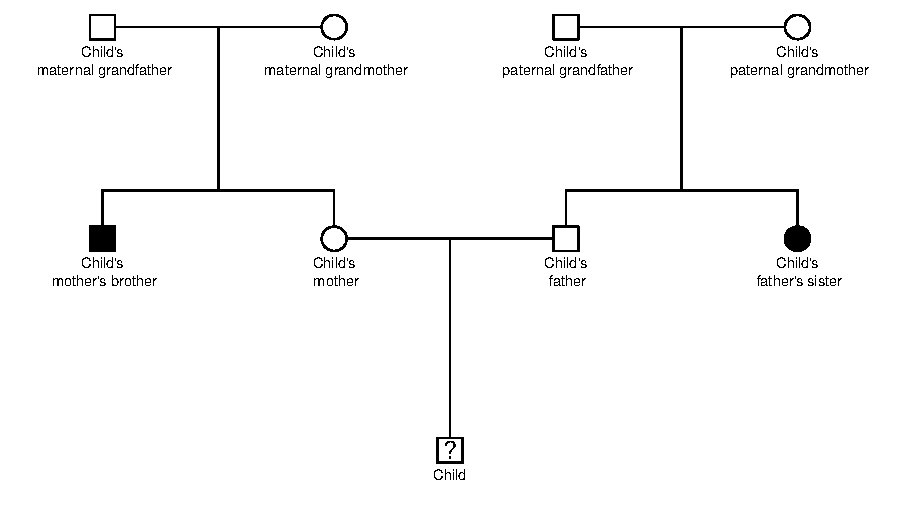
\includegraphics[width=0.85\linewidth]{./figures/pedigree-gp-p-off}}
\end{center}

When these inferences have been made, the problem is reduced to an application of the product rule. The only way in which the man and woman can have a PKU child is if both of them are heterozygotes (it is obvious that they themselves do not have the disease). Both the grandparental matings are simple Mendelian monohybrid crosses expected to produce progeny in the following proportions:

\[
\begin{aligned}
&\frac{1}{4} P/P, \frac{1}{2} P/\_; & \text{Normal} \longrightarrow \frac{3}{4} \\
&\frac{1}{4} p/p; & \textrm{PKU} \longrightarrow \frac{1}{4}
\end{aligned}
\]

We know that the man and the woman are normal, and so the probability of each being a heterozygote is 2/3 because, within the P/\_ class, 2/3 are P/p and 1/3 are P/P. The probability of both the man and the woman being heterozygotes is 2/3 x 2/3 = 4/9. If both are heterozygous, then one-quarter of their children would have PKU, and so the probability that their first child will have PKU is 1/4 and the probability of their being heterozygous and of their first child's having PKU is 4/9 x 1/4 = 4/36 = 1/9, which is the answer.

\esolution

\equestions

\end{document}
